\section{The Large Hadron Collider}
The Large Hadron Collider (LHC) is the highest-energy particle collider ever constructed. Located at the European Organization for Nuclear Research (CERN) and housed in a \SI{27}{\km} ring approximately \SI{100}{\m} below the French/Swiss countryside, the LHC is designed to accelerate two counter-rotating beams of protons to \SI{7}{\TeV} (and sometimes beams of heavy ions to \SI{2.8}{\TeV}) and collide them at four points around the ring. Each collision point is instrumented with a dedicated detector: the ATLAS (A Toroidal LHC ApparatuS) and CMS (Compact Muon Solenoid) experiments are general purpose detectors designed to reconstruct the remnants of proton-proton collisions at the highest collision rates offered by the LHC, LHCb (LHC beauty) studies b-quark decays from proton-proton collisions produced at lower collision rates, and ALICE (A Large Ion Collider Experiment) studies heavy-ion collisions~\cite{lhc_machine}. Figure~\ref{lhc_layout} shows the location of each experiment around the LHC ring. The analysis presented in Chapter~\ref{displaced_leptons} utilizes proton-proton collision data collected by the CMS experiment, and the following discussion is focused accordingly.

\begin{figure}
\centering
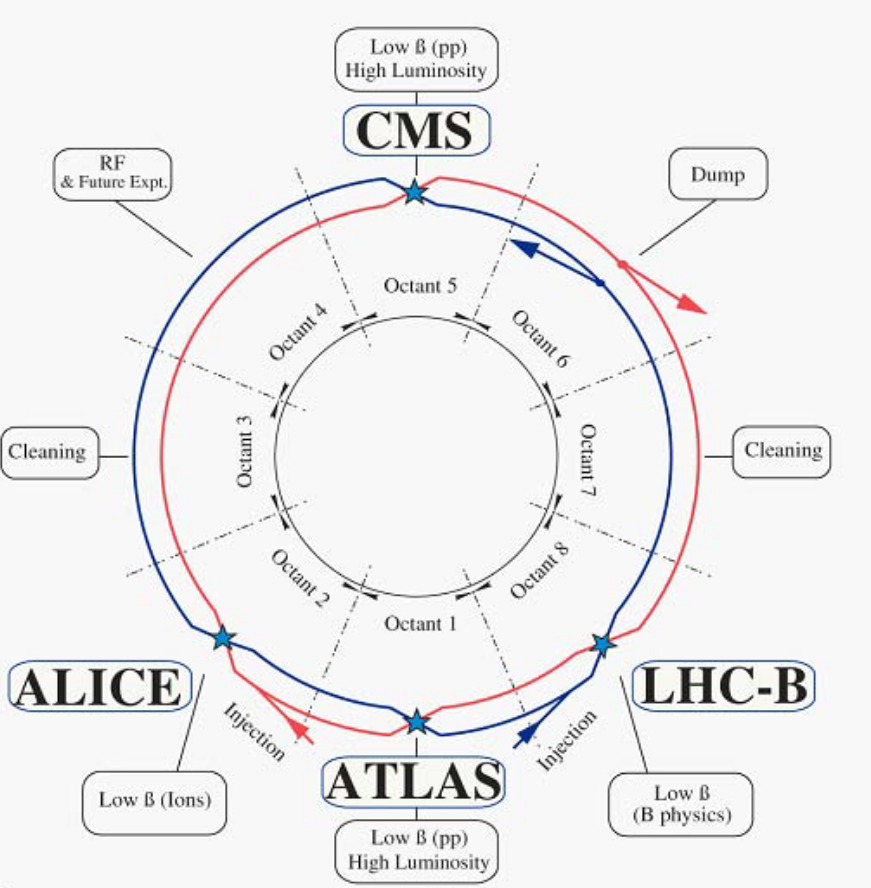
\includegraphics[width=0.5\textwidth]{figures/lhc_and_cms/lhc_layout.png}
\caption{Layout of the LHC experiments~\cite{lhc_machine}.}
\label{lhc_layout}
\end{figure}

\subsection{Injection chain}
The protons ultimately collided by the LHC must first travel through much of the CERN accelerator complex, which is diagrammed in Fig.~\ref{cern_accelerator_complex}. The \SI{6.5}{\TeV} proton beams relevant to this thesis start their journey as the nuclei of hydrogen atoms in a bottle of hydrogen gas. After having their electrons stripped away with an electric field, the protons are accelerated to an energy of \SI{50}{\MeV} with the Linac 2 linear accelerator~\cite{linac2}. The Proton Synchrotron Booster (PSB) next accelerates the protons to an energy of \SI{1.4}{\GeV} before injecting them into the Proton Synchrotron (PS)~\cite{psb}. The PS was the first synchrotron constructed at CERN and was the highest-energy particle accelerator in the world at the time of its first operation~\cite{cern_annual_report_1959}. Today, it accelerates protons to an energy of \SI{25}{\GeV} before passing them along to the Super Proton Synchrotron (SPS), which is the \SI{7}{\km} proton-antiproton collider at which the \PWpm\ and \cPZ\ bosons were discovered in 1983~\cite{sps}. As the final step in the LHC injection chain, SPS accelerates protons to an energy of \SI{450}{\GeV} before injecting them into the LHC~\cite{lhc_machine}.

\begin{figure}[hbtp]
\centering
\includegraphics[scale=0.4]{figures/lhc_and_cms/cern_accelerator_complex.png}
\caption{A diagram of the CERN accelerator complex. The analysis presented in Chapter~\ref{displaced_leptons} utilizes protons accelerated by LINAC 2, BOOSTER (also known as PSB), PS, SPS, and finally the LHC before their ultimate collision inside CMS \cite{cern_accelerator_complex}.}
\label{cern_accelerator_complex}
\end{figure}

\subsection{Main ring}
Maximizing the physics potential of the LHC requires simultaneously maximizing the collision energy and the number of interesting collisions per unit time. The main LHC ring is therefore designed to accelerate the \SI{450}{\GeV} protons it receives from SPS to \SI{7}{\GeV} and collimate them into intense beams to be collided at high rates. The number of interesting collisions per unit time is ultimately the product of the total cross section of the processes one deems interesting, $\sigma$, and the instantaneous luminosity, $L$, which is given by:
\begin{equation}
\label{lumi_eq}
L = \frac{N_{b}^{2} n_{b} f_{rev} \gamma_{r}}{4 \pi \epsilon_{n} \beta^{*}}F
\end{equation}
where the parameters are defined as in Table~\ref{lumi_params} ~\cite{lhc_machine}.

\begin{table}[h]
\noindent \centering{}
\caption{Luminosity parameters used in Eq.~\eqref{lumi_eq}.}
\label{lumi_params}
\begin{tabular}{cl}
\hline
Parameter & Description\\
\hline
$N_{b}$ & Number of particles per bunch\\
$n_{b}$ & Number of bunches per beam\\
$f_{rev}$ & Revolution frequency\\
$\gamma_{r}$ & Relativistic gamma factor\\
$\epsilon_{n}$ & Normalized transverse beam emittance\\
$\beta^{*}$ & Beta function at collision point\\
$F$ & Geometric luminosity reduction factor\\
\hline
\end{tabular}
\end{table}
% \FIXME: add 2016-2018 values?

The LHC is designed to deliver a maximum instantaneous luminosity of \linebreak[4] \SI{e34}{\cm\tothe{-2}\s\tothe{-1}} to ATLAS and CMS, but operational improvements, most notably a reduction in $\epsilon_{n}$ and $\beta^{*}$, have allowed the LHC to exceed this goal by up to a factor of approximately two in the 2016, 2017, and 2018 data-taking periods~\cite{lhc_run2_operation}. As shown in Fig.~\ref{lhc_lumi}, the total integrated luminosity delivered during this period is approximately a factor of five times greater than that of the 2011--2012 period.

Increasing the number of interesting collisions per unit time comes with the unfortunate side effect of increasing the total number of collisions in each bunch crossing. Due to storage and processing limitations, the CMS and ATLAS detectors only record data from the small subset of bunch crossings whose properties imply that they may contain interesting processes (see Section~\ref{trigger}). In a given bunch crossing, usually only one collision is considered interesting. The remaining collisions, referred to as ``pileup", add a layer of difficulty to collecting and analyzing the data while increasing the total radiation dose that the detectors must withstand.

The ability to produce high-energy proton collisions at such high rates depends on several impressive technological feats, notably the superconducting magnets that steer and shape the beams and the superconducting radio-frequency (RF) cavities that accelerate the protons and determine their bunch structure.

\begin{figure}
\centering
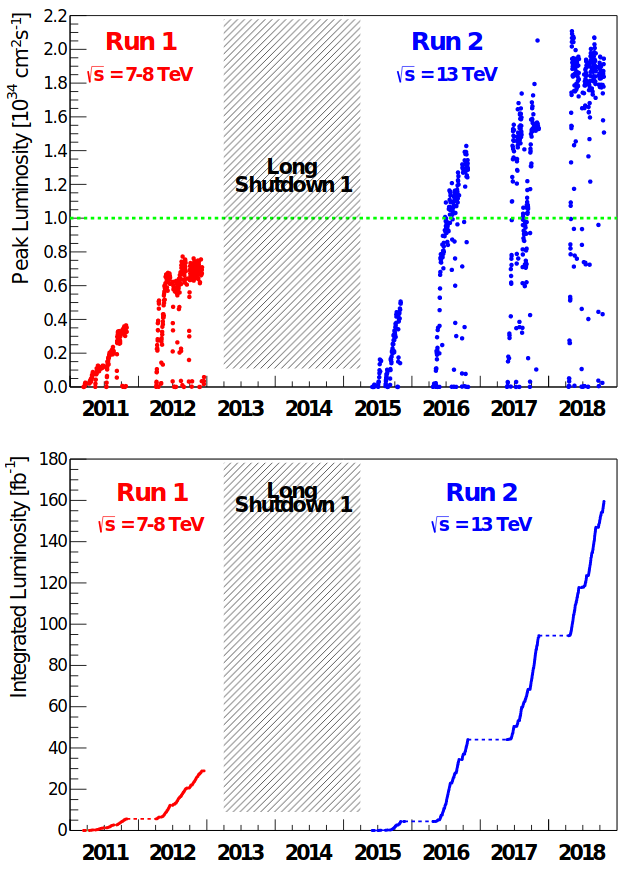
\includegraphics[width=0.6\textwidth]{figures/lhc_and_cms/lhc_lumi.png}
\caption{The peak instantaneous (top) and integrated (bottom) luminosity delivered by the LHC during proton operation between 2011 and 2018 \cite{lhc_run2_operation}.}
\label{lhc_lumi}
\end{figure}

\subsubsection{Superconducting magnets}
The LHC magnet system relies on superconducting NbTi magnets that are cooled to below \SI{2}{\K} with superfluid helium and are capable of producing fields in excess of \SI{8}{\tesla}. The design of the main dipole magnets that are responsible for keeping the beams in a circular trajectory is heavily influenced by the size of the LHC tunnel, which originally housed the Large Electron-Positron Collider (LEP). Unlike LEP, which collided particles and antiparticles, the LHC requires two separate beam pipes, each with its own dipole magnetic field. This requirement, along with the limited tunnel cross section, motivates the ``two-in-one" magnet design in which both superconducting magnets share a common cold mass and cryostat, as shown in Fig.~\ref{lhc_dipole}~\cite{lhc_machine}.

In addition to the main dipole magnets, the LHC also employs quadrupole magnets for beam focusing and sextupole, octupole, and decapole magnets to correct the field at the edges of the dipoles~\cite{lhc_machine}.

\begin{figure}
\centering
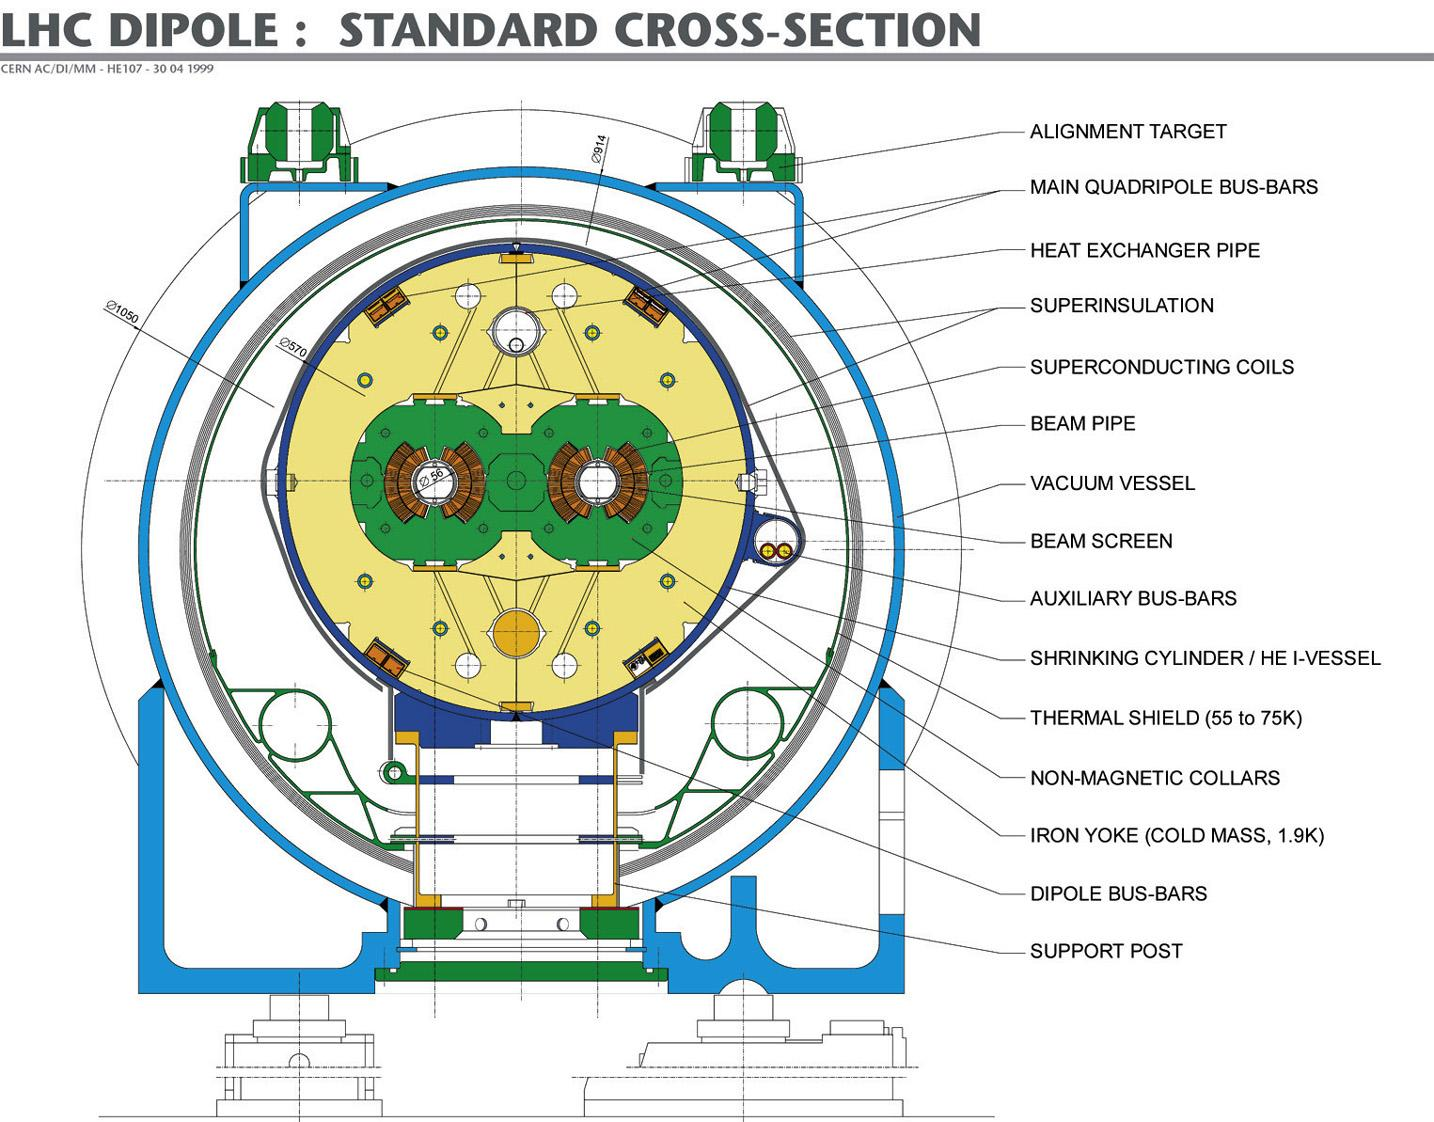
\includegraphics[width=0.8\textwidth]{figures/lhc_and_cms/lhc_dipole.jpg}
\caption{Diagram of an LHC dipole magnet in cross-section~\cite{lhc_dipole}.}
\label{lhc_dipole}
\end{figure}

\subsubsection{Radio-frequency cavities}
An RF superconducting cavity system is responsible for capturing the \SI{450}{\GeV} protons injected into the LHC from SPS, accelerating them to the full collision energy, defining their bunch structure, and storing them. The main RF system operates at \SI{400}{\MHz} and is located in Octant 4 (see Fig.\ref{lhc_layout}). Each RF cavity contains an oscillating electromagnetic field whose phase is synchronized with the arrival of the proton bunches such that the protons passing through the cavity always feel a force in the direction of their motion. The applied force naturally varies for protons that are slightly out of phase in such a way as to keep the protons tightly bunched in the longitudinal direction~\cite{lhc_machine}.

\pagebreak
